%%%%%%%%%%%%%%%%%%%%%%%%%%%%%%%%%%%%%%%%%%%%%%%%%%%%%%%%%%%%%%%%%%%%%%%%%%%%%%%%%%
\begin{frame}[fragile]\frametitle{}
\begin{center}
{\Large Application of knowledge }
\end{center}
\end{frame}


%%%%%%%%%%%%%%%%%%%%%%%%%%%%%%%%%%%%%%%%%%%%%%%%%%%%%%%%%%%
\begin{frame}[fragile]\frametitle{Application of Knowledge: Marks and Format}
\begin{itemize}
\item \textbf{Marks}: 10 of the 140 practical marks.
\item \textbf{Where it is assessed}: inside the practical assessment, which lasts at most one hour per candidate.
\item \textbf{What it asks}: use what you know about the protocol, the practices and the learner to decide what to teach, and explain why.
\item \textbf{Preparation}: prepare a few real cases, such as a beginner, an older adult and a person with a stiff back, and say what you would keep, change or leave out.
\end{itemize}
{\tiny (Ref: YCB, Guidelines for Yoga Professionals, Version 0.2; the case examples are study suggestions, not official questions)}
\end{frame}

%%%%%%%%%%%%%%%%%%%%%%%%%%%%%%%%%%%%%%%%%%%%%%%%%%%%%%%%%%%
\begin{frame}[fragile]\frametitle{Application of Knowledge as Yoga Protocol Instructor}
\begin{columns}
    \begin{column}[T]{0.5\linewidth}
      \begin{itemize}
        \item \textbf{Protocol Implementation}: Apply \textbf{standard yoga protocols} in practice.
        \item \textbf{Customized Instruction}: Tailor \textbf{instructions} based on \textbf{student needs}.
        \item \textbf{Assessment Techniques}: Utilize \textbf{assessment methods} to gauge \textbf{progress}.
        \item \textbf{Lesson Adaptation}: Adjust \textbf{lessons} based on \textbf{feedback} and \textbf{observation}.
        \item \textbf{Effective Communication}: Use \textbf{clear communication} to convey \textbf{instructions} and \textbf{guidance}.
      \end{itemize}
    \end{column}
    \begin{column}[T]{0.5\linewidth}
        \begin{center}
        % FIG ycb1-fig-application-of-knowledge | now: images/ycb1_application_of_knowledge.png | final: workshops/YCB1/images/new/ycb1_application_of_knowledge_new.pdf | register: books/YCB1/docs/image_register.csv
        % PROMPT SP-DIAGRAM (common text: books/YCB1/docs/image_system_prompt.md) | Used in block ycb1-pa-application-of-knowledge, frame 'Application of Knowledge as Yoga Protocol Instructor'. Concept diagram: Application of Knowledge as Yoga Protocol Instructor. Boxes, circles and arrows only, drawn from the structure given in the notes block (the names and their order are listed there); Sanskrit terms in Roman letters with the English meaning in brackets, nothing else added. Flat colours that still read in grayscale. Best redrawn later in TikZ. Aspect ratio 4:3. Check before use: author and the Sanskrit check in the notes.
        % NEW-PIC (uncomment to show the new picture beside the original; comment the original only after review) \includegraphics[width=0.35\linewidth,keepaspectratio]{new/ycb1_application_of_knowledge_new.pdf}
        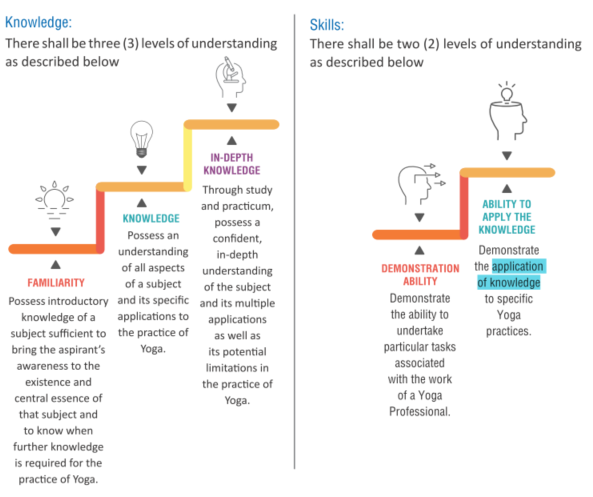
\includegraphics[width=\linewidth,keepaspectratio]{ycb1_application_of_knowledge}

		{\tiny (Ref: Certification  of Yoga Professionals Official Guidebook For Level I (Instructor))}		
		
        \end{center}	
    \end{column}
\end{columns}
\end{frame}

